\documentclass[11pt,a4paper]{article}
\usepackage[margin=2.2cm]{geometry}
\usepackage[T1]{fontenc}
\usepackage{booktabs}
\usepackage{longtable}
\usepackage{array}
\usepackage{xcolor}
\usepackage{titlesec}
\usepackage{enumitem}
\usepackage{graphicx}
\usepackage{amsmath}
\usepackage{amssymb}
\usepackage{listings}
\usepackage[hidelinks]{hyperref}

\definecolor{good}{HTML}{1B7F3B}
\definecolor{warn}{HTML}{B26B00}
\definecolor{bad}{HTML}{B3261E}
\definecolor{grey}{HTML}{666666}
\definecolor{lst}{HTML}{F5F5F5}

\newcommand{\code}[1]{\texttt{\small #1}}
\newcommand{\gd}[1]{\textcolor{good}{\textbf{#1}}}
\newcommand{\bd}[1]{\textcolor{bad}{\textbf{#1}}}
\newcommand{\wn}[1]{\textcolor{warn}{\textbf{#1}}}

\titleformat{\section}{\large\bfseries}{\thesection.}{0.6em}{}
\titleformat{\subsection}{\normalsize\bfseries}{\thesubsection}{0.6em}{}
\setlist{leftmargin=1.2em,itemsep=2pt,topsep=3pt}

\lstset{basicstyle=\ttfamily\scriptsize, backgroundcolor=\color{lst}, frame=none,
        numbers=left, numberstyle=\tiny\color{grey}, xleftmargin=2.4em, framexleftmargin=2em,
        columns=fullflexible, breaklines=true, showstringspaces=false, language=Python,
        keywordstyle=\color{black}, commentstyle=\color{grey}\itshape, aboveskip=4pt,
        belowskip=4pt}

% GENERATED by tools/mpm_warp_note.py -- do not edit
\newcommand{\tblScatterDefault}{%
\begin{tabular}{@{}llrrrr@{}}
\toprule
aten op & shape & dtype & \multicolumn{1}{c}{each} & \multicolumn{1}{c}{$\times$} & \multicolumn{1}{c}{total} \\
\midrule
\code{clone} & \code{[945000, 27, 3, 3]} & float32 & 918.5\,MB & 1 & 918.5\,MB \\
\code{mul} & \code{[945000, 27]} & float32 & 102.1\,MB & 6 & 612.4\,MB \\
\code{add} & \code{[945000, 27, 3]} & int64 & 612.4\,MB & 1 & 612.4\,MB \\
\code{clamp} & \code{[945000, 27]} & int64 & 204.1\,MB & 3 & 612.4\,MB \\
\code{mul} & \code{[945000, 27, 3]} & float32 & 306.2\,MB & 2 & 612.4\,MB \\
\code{mul} & \code{[945000, 27]} & int64 & 204.1\,MB & 2 & 408.2\,MB \\
\code{add} & \code{[945000, 27]} & int64 & 204.1\,MB & 2 & 408.2\,MB \\
\code{index} & \code{[945000, 27]} & float32 & 102.1\,MB & 3 & 306.2\,MB \\
\code{sub} & \code{[945000, 27, 3]} & float32 & 306.2\,MB & 1 & 306.2\,MB \\
\code{bmm} & \code{[25515000, 3, 1]} & float32 & 306.2\,MB & 1 & 306.2\,MB \\
\code{add} & \code{[945000, 27, 3]} & float32 & 306.2\,MB & 1 & 306.2\,MB \\
\code{index\_select} & \code{[945000, 3, 3]} & float32 & 34.0\,MB & 8 & 272.2\,MB \\
\code{mul} & \code{[945000, 3, 3]} & float32 & 34.0\,MB & 8 & 272.2\,MB \\
\code{add} & \code{[945000, 3, 3]} & float32 & 34.0\,MB & 6 & 204.1\,MB \\
\code{linalg\_cross} & \code{[945000, 3, 3]} & float32 & 34.0\,MB & 4 & 136.1\,MB \\
\code{div} & \code{[945000, 3, 3]} & float32 & 34.0\,MB & 4 & 136.1\,MB \\
\code{mul} & \code{[945000, 3]} & float32 & 11.3\,MB & 10 & 113.4\,MB \\
\code{ones} & \code{[945000, 27]} & float32 & 102.1\,MB & 1 & 102.1\,MB \\
\code{sub} & \code{[945000, 3]} & float32 & 11.3\,MB & 5 & 56.7\,MB \\
\midrule
\multicolumn{5}{@{}l}{\textbf{all allocating ops}} & \textbf{7177\,MB} \\
\multicolumn{5}{@{}l}{per particle} & \textbf{7594\,B} \\
\multicolumn{5}{@{}l}{$\div$ essential (864\,B)} & \textbf{8.8$\times$} \\
\bottomrule
\end{tabular}
}

\newcommand{\tblGatherDefault}{%
\begin{tabular}{@{}llrrrr@{}}
\toprule
aten op & shape & dtype & \multicolumn{1}{c}{each} & \multicolumn{1}{c}{$\times$} & \multicolumn{1}{c}{total} \\
\midrule
\code{bmm} & \code{[25515000, 3, 3]} & float32 & 918.5\,MB & 1 & 918.5\,MB \\
\code{mul} & \code{[945000, 27, 3, 3]} & float32 & 918.5\,MB & 1 & 918.5\,MB \\
\code{add} & \code{[945000, 27, 3]} & int64 & 612.4\,MB & 1 & 612.4\,MB \\
\code{clamp} & \code{[945000, 27]} & int64 & 204.1\,MB & 3 & 612.4\,MB \\
\code{mul} & \code{[945000, 27]} & int64 & 204.1\,MB & 2 & 408.2\,MB \\
\code{add} & \code{[945000, 27]} & int64 & 204.1\,MB & 2 & 408.2\,MB \\
\code{index} & \code{[945000, 27]} & float32 & 102.1\,MB & 3 & 306.2\,MB \\
\code{mul} & \code{[945000, 27]} & float32 & 102.1\,MB & 3 & 306.2\,MB \\
\code{index} & \code{[25515000, 3]} & float32 & 306.2\,MB & 1 & 306.2\,MB \\
\code{mul} & \code{[945000, 27, 3]} & float32 & 306.2\,MB & 1 & 306.2\,MB \\
\code{sub} & \code{[945000, 27, 3]} & float32 & 306.2\,MB & 1 & 306.2\,MB \\
\code{ones} & \code{[945000, 27]} & float32 & 102.1\,MB & 1 & 102.1\,MB \\
\code{mul} & \code{[945000, 3]} & float32 & 11.3\,MB & 6 & 68.0\,MB \\
\code{sub} & \code{[945000, 3]} & float32 & 11.3\,MB & 4 & 45.4\,MB \\
\midrule
\multicolumn{5}{@{}l}{\textbf{all allocating ops}} & \textbf{6060\,MB} \\
\multicolumn{5}{@{}l}{per particle} & \textbf{6413\,B} \\
\multicolumn{5}{@{}l}{$\div$ essential (864\,B)} & \textbf{7.4$\times$} \\
\bottomrule
\end{tabular}
}

\newcommand{\Ntrace}{945\,000}

\newcommand{\mbstrain}{296}

\newcommand{\bpstrain}{313}

\newcommand{\mbscatter}{7177}

\newcommand{\bpscatter}{7594}

\newcommand{\mbgridupdate}{142}

\newcommand{\bpgridupdate}{151}

\newcommand{\mbgather}{6060}

\newcommand{\bpgather}{6413}

\newcommand{\mbtotal}{13675}

\newcommand{\ampltotal}{16.7}

\newcommand{\mbtotalwarp}{438}

\newcommand{\ampltotalwarp}{0.5}

\newcommand{\warpfusedmb}{0}

\newcommand{\tblAblation}{%
\begin{tabular}{@{}llrrr@{}}
\toprule
\code{mpm\_scatter} & \code{mpm\_gather} & ms/frame & peak & speedup \\
\midrule
default & default & 1150.8 & 2.94\,GiB & 1.0$\times$ \\
\textbf{warp} & default & 466.9 & 2.80\,GiB & 2.5$\times$ \\
default & \textbf{warp} & 767.8 & 2.94\,GiB & 1.5$\times$ \\
\textbf{warp} & \textbf{warp} & 79.4 & 0.35\,GiB & 14.5$\times$ \\
\textbf{warp} & \textbf{warp} \;{\footnotesize +capture} & 52.2 & 0.55\,GiB & 22.0$\times$ \\
\bottomrule
\end{tabular}
}

\newcommand{\tblSweepAsix}{%
\begin{tabular}{@{}rrrrrr@{}}
\toprule
particles & sub & ms/frame & ms/substep & GB/s & \% peak \\
\midrule
945\,000 & 7 & 77.8 & 11.12 & 73.4 & 9.6\% \\
1\,999\,998 & 7 & 161.8 & 23.12 & 74.7 & 9.7\% \\
4\,999\,995 & 7 & 402.1 & 57.44 & 75.2 & 9.8\% \\
9\,999\,990 & 7 & 784.9 & 112.13 & 77.1 & 10.0\% \\
20\,000\,007 & 7 & 1614.1 & 230.58 & 74.9 & 9.8\% \\
100\,000\,008 & 7 & 7968.9 & 1138.42 & 75.9 & 9.9\% \\
\bottomrule
\end{tabular}
}

\newcommand{\tblSweepAhun}{%
\begin{tabular}{@{}rrrrrr@{}}
\toprule
particles & sub & ms/frame & ms/substep & GB/s & \% peak \\
\midrule
500\,013 & 7 & 24.0 & 3.42 & 126.2 & 8.1\% \\
999\,999 & 7 & 46.7 & 6.67 & 129.6 & 8.3\% \\
4\,999\,995 & 7 & 229.8 & 32.84 & 131.6 & 8.5\% \\
\bottomrule
\end{tabular}
}

\newcommand{\tblSweepAhunPlain}{%
\begin{tabular}{@{}rrrrrr@{}}
\toprule
particles & sub & ms/frame & ms/substep & GB/s & \% peak \\
\midrule
500\,013 & 7 & 40.7 & 5.82 & 74.2 & 4.8\% \\
999\,999 & 7 & 71.3 & 10.18 & 84.9 & 5.5\% \\
4\,999\,995 & 7 & 378.5 & 54.07 & 79.9 & 5.1\% \\
\bottomrule
\end{tabular}
}

% GENERATED by tools/mpm_perf.py --latex -- do not edit
\newcommand{\tblImplSweep}{%
\begin{tabular}{@{}llrrrrc@{}}
\toprule
scene & implementation & \multicolumn{1}{c}{ms/frame} & \multicolumn{1}{c}{ms/substep} & \multicolumn{1}{c}{ns/p-substep} & \multicolumn{1}{c}{peak GiB} & capture \\
\midrule
\multicolumn{7}{@{}l}{\emph{si\_waterfall, 570,760 particles, 13 substeps/frame --- NVIDIA A100-SXM4-80GB}} \\
& \code{warpgrid\_cap} & 31.8 & 2.45 & 4.29 & 0.32 & yes \\
& \code{warpgrid\_eager} & 32.4 & 2.49 & 4.37 & 0.22 & -- \\
& \code{warp\_cap} & 38.7 & 2.98 & 5.22 & 0.34 & yes \\
& \code{warp\_eager} & 41.6 & 3.20 & 5.61 & 0.24 & -- \\
& \code{torch\_loop27\_cap} & 434.0 & 33.38 & 58.49 & 1.55 & yes \\
& \code{torch\_loop27\_eager} & 450.1 & 34.62 & 60.66 & 1.39 & -- \\
& \code{torch\_cap} & 958.9 & 73.76 & 129.23 & 1.91 & yes \\
& \code{torch\_eager} & 973.8 & 74.90 & 131.24 & 1.74 & -- \\
\midrule
\multicolumn{7}{@{}l}{\emph{si\_waterfall, 570,760 particles, 13 substeps/frame --- NVIDIA RTX A6000}} \\
& \code{warpgrid\_cap} & 35.0 & 2.69 & 4.72 & 0.32 & yes \\
& \code{warpgrid\_eager} & 35.3 & 2.71 & 4.75 & 0.22 & -- \\
& \code{warp\_cap} & 52.7 & 4.05 & 7.10 & 0.34 & yes \\
& \code{warp\_eager} & 55.1 & 4.24 & 7.42 & 0.24 & -- \\
& \code{torch\_loop27\_cap} & 627.8 & 48.29 & 84.61 & 1.55 & yes \\
& \code{torch\_loop27\_eager} & 640.4 & 49.26 & 86.31 & 1.39 & -- \\
& \code{torch\_cap} & 952.2 & 73.25 & 128.33 & 1.91 & yes \\
& \code{torch\_eager} & 962.9 & 74.07 & 129.77 & 1.74 & -- \\
\midrule
\multicolumn{7}{@{}l}{\emph{si\_waterfall\_5m, 5,000,000 particles, 26 substeps/frame --- NVIDIA A100-SXM4-80GB}} \\
& \code{warpgrid\_cap} & 441.0 & 16.96 & 3.39 & 2.71 & yes \\
& \code{warpgrid\_eager} & 442.1 & 17.00 & 3.40 & 1.90 & -- \\
& \code{warp\_cap} & 590.5 & 22.71 & 4.54 & 2.81 & yes \\
& \code{warp\_eager} & 601.4 & 23.13 & 4.63 & 2.01 & -- \\
& \code{torch\_loop27\_cap} & 7622.6 & 293.18 & 58.63 & 12.75 & yes \\
& \code{torch\_loop27\_eager} & 7696.2 & 296.01 & 59.20 & 11.88 & -- \\
& \code{torch\_cap} & 16839.3 & 647.67 & 129.53 & 15.91 & yes \\
& \code{torch\_eager} & 16965.5 & 652.52 & 130.50 & 14.93 & -- \\
\midrule
\multicolumn{7}{@{}l}{\emph{si\_waterfall\_5m, 5,000,000 particles, 26 substeps/frame --- NVIDIA RTX A6000}} \\
& \code{warpgrid\_cap} & 933.0 & 35.88 & 7.18 & 2.71 & yes \\
& \code{warpgrid\_eager} & 934.6 & 35.95 & 7.19 & 1.90 & -- \\
& \code{warp\_cap} & 1267.5 & 48.75 & 9.75 & 2.81 & yes \\
& \code{warp\_eager} & 1272.6 & 48.95 & 9.79 & 2.01 & -- \\
& \code{torch\_loop27\_cap} & 10913.0 & 419.73 & 83.95 & 12.75 & yes \\
& \code{torch\_loop27\_eager} & 10974.1 & 422.08 & 84.42 & 11.88 & -- \\
& \code{torch\_cap} & 16668.8 & 641.11 & 128.22 & 15.91 & yes \\
& \code{torch\_eager} & 16767.7 & 644.91 & 128.98 & 14.93 & -- \\
\bottomrule
\end{tabular}}

\newcommand{\tblScaling}{%
\begin{tabular}{@{}lrrrrrr@{}}
\toprule
GPU & \multicolumn{1}{c}{particles} & \multicolumn{1}{c}{$n_{\mathrm{grid}}$} & \multicolumn{1}{c}{substeps} & \multicolumn{1}{c}{ms/frame} & \multicolumn{1}{c}{ns/p-substep} & \multicolumn{1}{c}{peak GiB} \\
\midrule
H100 80GB HBM3 & 200\,M & 192 & 13 & 5410 & 2.08 & 51.7 \\
B300 SXM6 AC & 800\,M & 296 & 20 & 14127 & 0.88 & 206.8 \\
B300 SXM6 AC & 1000\,M & 320 & 22 & 18918 & 0.86 & 258.4 \\
\bottomrule
\end{tabular}}



\title{\vspace{-1.6cm}\textbf{Two implementations of the same MPM}\\[3pt]
\large \code{default} against \code{warp}: where the time goes, and why}
\author{}
\date{}

\begin{document}
\maketitle
\vspace{-1.1cm}

\section{The result}

The four MLS-MPM operators --- \code{mpm\_strain}, \code{mpm\_scatter}, \code{mpm\_grid\_update},
\code{mpm\_gather} --- exist in two forms a spec picks by name on the \code{implementation} axis.
\code{default} is pure PyTorch: 2D and 3D, CPU or CUDA, and differentiable in use, not merely in
principle (\code{engine.run(\ldots, grad=True)} keeps the tape across a rollout and
\code{discovery\_cardio\_mpm/train.py} backpropagates through exactly these four). \code{warp} is
one NVIDIA Warp kernel per operator, 3D and CUDA only. Same equations, so they sit on the
\code{implementation} axis and not the \code{model} axis: swapping one for the other asserts the
physics did not change, and \S6 tests that assertion.

\paragraph{On \code{si\_waterfall} --- 570\,760 particles, $96^3$ grid, 13 substeps, A100:}
\bd{973.8\,ms/frame} for \code{default} against \gd{31.8\,ms/frame} for \code{warp} with the grid
solve fused and the substep captured --- \gd{$30.6\times$}. At 5\,M particles on a $192^3$ grid it is
16\,965 against 441\,ms, \gd{$38.5\times$}. One RTX A6000 runs 150\,M particles; one B300 runs
\gd{one billion}.

\paragraph{The mechanism is traffic, not memory held.} \textbf{Traffic here means bytes moved
between the GPU's DRAM and its compute units} --- read into the streaming multiprocessors and written
back out. It is the quantity a memory-bound kernel actually spends its time on. Every intermediate
tensor an operator allocates is one DRAM write plus at least one DRAM read by whatever consumes it;
a value held in a register never leaves the chip and costs none. \code{default}'s gather materialises
two $[N,27,3,3]$ tensors --- 918.5\,MB each at 945\,k particles --- to produce a $[N,3,3]$ result of
34.0\,MB. The Warp kernel accumulates the same sum in nine registers and writes none of it.

It is tempting to read the peak-memory drop (2.94\,GiB $\to$ 0.35\,GiB) as the cause. \textbf{Peak
memory is a stock and traffic is a flow}, and \S5.2 separates them: on one substep of the gather at
570\,760 particles, the batched form allocates \bd{3511.9\,MB} and the loop form \gd{1924.7\,MB} ---
$1.82\times$ less traffic, $1.25\times$ less peak, and $3.70\times$ less time. Time tracks the flow,
not the stock.

\begin{figure}[t]
\centering
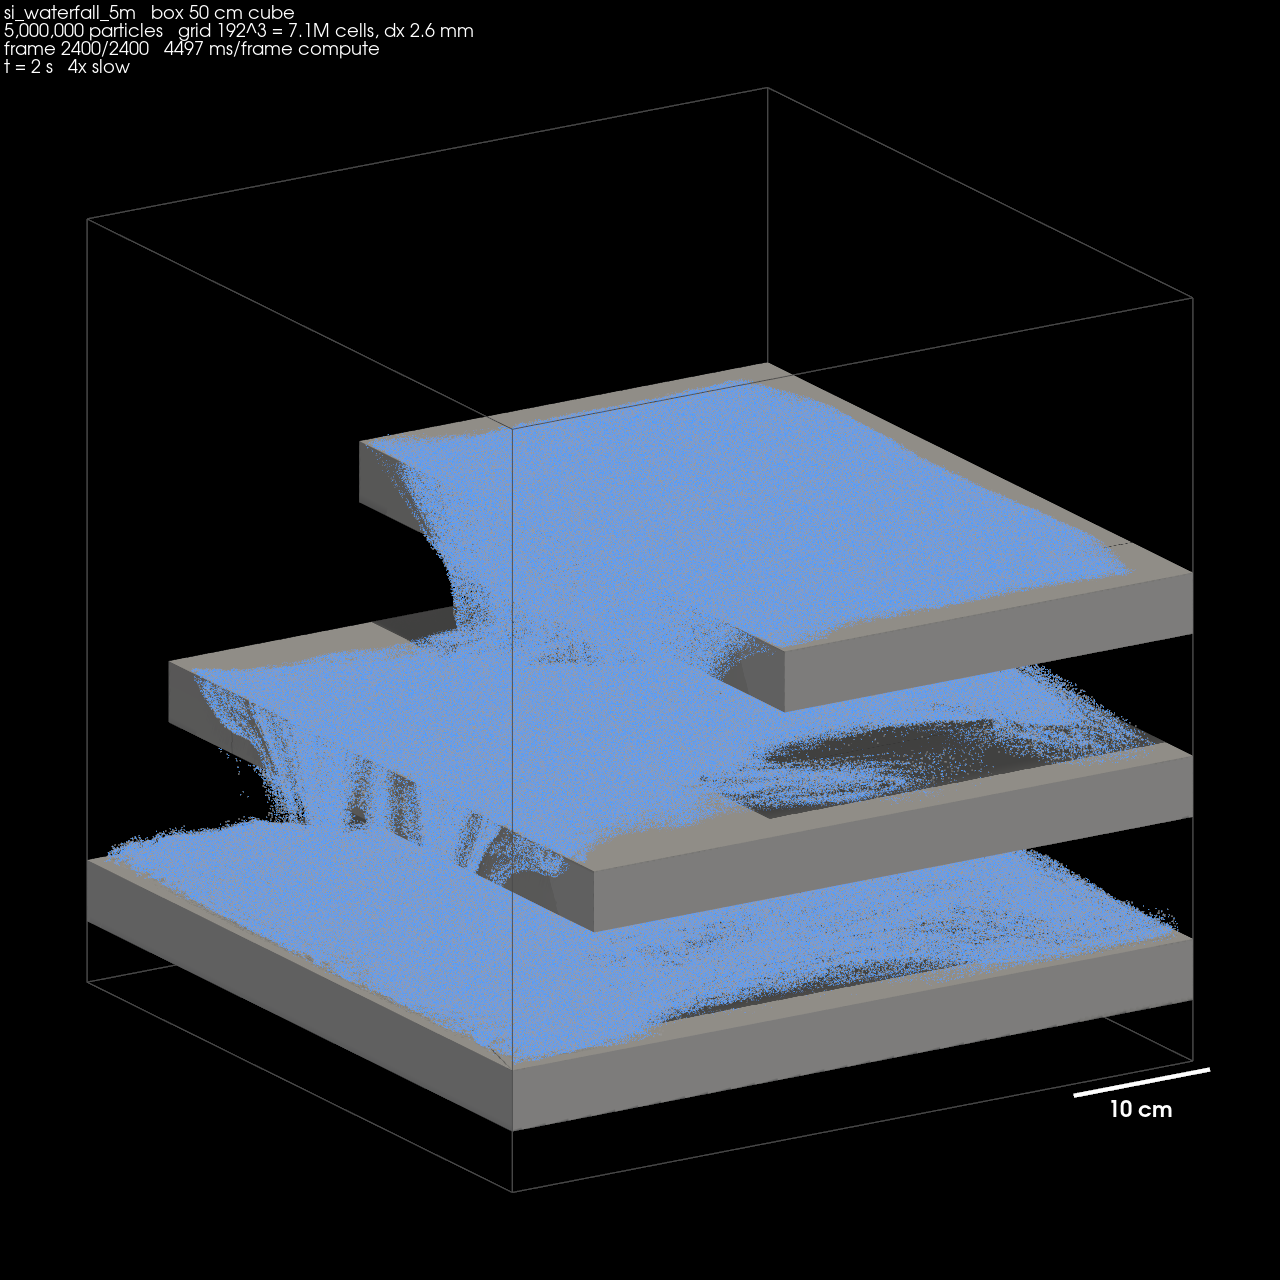
\includegraphics[width=0.72\textwidth]{figures/si_waterfall_5m}
\caption{\code{si\_waterfall\_5m}: 5\,000\,000 particles of water in a 50\,cm cube on a $192^3$ grid
($\Delta x = 2.6$\,mm), 26 substeps per frame, at $t=2$\,s. Every particle is simulated; the picture
is taken off the GPU as the run proceeds. This spec is one of the two the sweep in \S7 uses, and it
is dimensional --- the box, the scale bar and $\Delta x$ are in real units, so \code{4497\,ms/frame}
buys 2 seconds of water rather than 2 seconds of nothing in particular.}
\end{figure}

\section{The cycle}

MLS-MPM carries material on particles $p$ and solves on a background grid $i$ thrown away every
substep. With $\Delta x$ the cell size, $w_{ip}$ the quadratic B-spline weight of node $i$ at
particle $p$, and $\mathbf{x}_{ip}=\mathbf{x}_i-\mathbf{x}_p$:

\begin{align}
\textbf{strain}\quad & \mathbf{F}_p \leftarrow (\mathbf{I}+\Delta t\,\mathbf{C}_p)\,\mathbf{F}_p \\
\textbf{scatter}\quad & m_i = \sum_p w_{ip} m_p,
  \qquad (m\mathbf{v})_i = \sum_p w_{ip}\big[m_p\mathbf{v}_p + \mathbf{A}_p\,\mathbf{x}_{ip}\big] \\
& \mathbf{A}_p = -\tfrac{4\Delta t}{\Delta x^{2}}V_p^{0}\,\boldsymbol{\sigma}_p + m_p\mathbf{C}_p,
  \qquad \boldsymbol{\sigma}_p = 2\mu(\mathbf{F}_p-\mathbf{R}_p)\mathbf{F}_p^{\!\top}
   + \lambda J(J-1)\mathbf{I} \\
\textbf{grid}\quad & \mathbf{v}_i = (m\mathbf{v})_i / \max(m_i,\epsilon),
  \quad\text{then gravity, walls, plates, surface tension} \\
\textbf{gather}\quad & \mathbf{v}_p = \sum_i w_{ip}\mathbf{v}_i,
  \qquad \mathbf{C}_p = \tfrac{4}{\Delta x}\sum_i w_{ip}\,
    \mathbf{v}_i \otimes (\mathbf{o}_i - \mathbf{f}_p),
  \qquad \mathbf{x}_p \leftarrow \mathbf{x}_p + \Delta t\,\mathbf{v}_p
\end{align}

$\mathbf{F}_p$ is the deformation gradient, one $3{\times}3$ per particle: the Jacobian of the map
from a particle's reference position to its current one, carrying accumulated stretch, shear and
rotation since $t=0$. $\mathbf{R}_p$ is its rotation part and $J=\det\mathbf{F}_p$ the volume ratio.
$\mathbf{o}_i-\mathbf{f}_p$ is $\mathbf{x}_{ip}$ in cell units. \textbf{The stencil is $3^3=27$
nodes}, because a quadratic B-spline spans three cells per axis and three dimensions multiply. Every
per-particle cost below carries that 27.

\paragraph{The contract both sign.} \code{mpm\_scatter} reads \code{pos, vel, C, F, mass, mu, la,
pvol} and the parent's acceleration, and accumulates into \code{mpm\_grid.m} and \code{.mv} in place.
It must \textbf{not} touch \code{F}: an early attempt fused the strain update into the scatter for
free and advanced \code{F} twice per substep --- grid mass still agreed to eleven digits while
\code{F} disagreed at $3.3\times10^{-4}$. \code{mpm\_gather} reads \code{mpm\_grid.v}, writes
\code{pos}, \code{vel}, \code{C} in place, and leaves dormant particles where they are.

\section{Why \code{default} is slow}

The gather is the shorter operator and makes the point completely. $N$ is the particle count,
$S=27$, $D=3$; sizes are at $N=\Ntrace$.

\begin{lstlisting}[numbers=none]
fx, weight, flat = bspline(X, inv_dx, offsets, g.shape, periodic)
    gpos   = base[:,None,:] + oidx[None]                         # [N,27,3] i64  612.4 MB
    flat   = ((c0 * ny) + c1) * nz + c2                          # [N,27]   i64  204.1 MB x4
gvn = g.v[flat].view(p.n, S, D)                                  # [N,27,3] f32  306.2 MB
new_V = (weight[..., None] * gvn).sum(1)                         # [N,27,3] f32  306.2 MB
dpos_grid = offsets[None] - fx[:, None, :]                       # [N,27,3] f32  306.2 MB
new_C = 4*inv_dx*(weight[...,None,None] *
        (gvn[...,:,None] @ dpos_grid[...,None,:])).sum(1)        # [N,27,3,3] f32 918.5 MB x2
\end{lstlisting}

\noindent
The last line is the whole story. That expression is $N\times27$ independent $3{\times}1$ by
$1{\times}3$ outer products, and PyTorch has no way to say ``form this $3{\times}3$, weight it, add
it to a running sum, discard it''. It must materialise all $N\times27$: write \gd{918.5\,MB}, read it
back to multiply by \code{weight}, write \gd{another 918.5\,MB}, read that back to reduce over the
stencil axis, and only then produce the $[N,3,3]$ anyone wanted --- \gd{34.0\,MB}. \textbf{The useful
output is 1.8\% of the traffic spent producing it.}

\subsection{The full bill, measured}

The listing is read off the source; the tables are measured. A \code{TorchDispatchMode} records every
\code{aten} call one real substep makes and the shape and dtype of everything it allocates ---
including what the source never names: broadcast temporaries, the \code{index} gathers hiding behind
\code{w[:, oidx[:,k], k]}, the int64 index arithmetic. Views are excluded, since they move nothing
and counting them would inflate \code{default}'s bill with bytes it never touches. Rows below 40\,MB
are omitted; totals include everything.

\begin{center}
\footnotesize
\textbf{\code{mpm\_gather}, \code{default}} \quad ($N=\Ntrace$, one substep)\\[2pt]
\tblGatherDefault
\end{center}

\begin{center}
\footnotesize
\textbf{\code{mpm\_scatter}, \code{default}} \quad (same substep)\\[2pt]
\tblScatterDefault
\end{center}

\noindent
Per particle per substep the four \code{default} operators allocate \bd{\bpstrain\,B} $+$
\bd{\bpscatter\,B} $+$ \bd{\bpgridupdate\,B} $+$ \bd{\bpgather\,B}. The \emph{essential} traffic ---
what any correct MLS-MPM must move --- is 216 floats $=864$\,B: read
\code{pos/vel/C/F/mass/mu/la}, scatter mass and momentum to 27 nodes, gather velocity back from 27.
\code{default} moves \bd{\ampltotal$\times$} the algorithm's requirement, and the two
$[N,27,3,3]$ tensors are most of it.

\section{Why \code{warp} is fast}

One thread per particle. Everything the tables list as a tensor is a local variable, and a local
variable in a CUDA thread is a register, which is not memory.

\paragraph{Nothing is ever 27 wide.} A thread has $\approx$64 registers --- nowhere near enough for
27 copies of (weight, node velocity, offset). The loop \emph{visits} the 27 nodes one at a time and
accumulates. Only \code{newv} (3 floats) and \code{newC} (9 floats) persist across iterations; each
node's weight, velocity and offset live for one iteration. The register cost is $O(1)$ in the stencil
size, not $O(27)$ --- exactly what PyTorch cannot express, having no way to form a value, add it to a
running sum and discard it, and so making the loop a tensor axis instead.

\code{ptxas -arch=sm\_86 -O3 --verbose} confirms the arithmetic fits: \gd{64 registers, 0 bytes stack
frame, 0 spill stores, 0 spill loads} for both \code{g2p} and \code{p2g\_atomic}. \textbf{Zero spill
is the load-bearing number}: had the working set exceeded the register file, the compiler would have
pushed the overflow to local memory --- global memory under another name --- and the fusion would
have bought nothing.

\begin{lstlisting}[numbers=none]
@wp.kernel                                    # src/plexus/operators/mpm_warp.py:193
def g2p(X, STATE, C, GV, OCC, LIQ, pa, va, ngx, ngy, ngz, dx, dt, ...):
    p = wp.tid()                              # one thread per particle
    newv = wp.vec3(0,0,0)                                  # vec3   -> 3 registers
    newC = wp.mat33(0,...,0)                               # mat33  -> 9 registers
    for i in range(3):                        # the 27-node stencil, UNROLLED by the compiler
      for j in range(3):
        for k in range(3):
          w    = wi*wj*wk                     #   the [N,27] `weight` tensor: 1 register
          gv   = GV[(gi*ngy + gj)*ngz + gk]   #   the [N,27,3] `gvn` tensor: 3 registers
          dpos = wp.vec3(i-fx[0], j-fx[1], k-fx[2])   #   the [N,27,3] `dpos_grid`: 3 registers
          newv = newv + w*gv                          #   the [N,27,3] product: never exists
          newC = newC + (4*inv_dx*w)*wp.outer(gv, dpos)  # the [N,27,3,3]: NEVER EXISTS
    STATE[p, pa+0..2] = xn ; STATE[p, va+0..2] = newv ; C[p] = newC   # the only writes
\end{lstlisting}

\begin{center}
\footnotesize
\begin{tabular}{@{}lrrl@{}}
\toprule
quantity & \code{default} tensor & at $N=\Ntrace$ & \code{warp} \\
\midrule
B-spline weights per axis     & \code{[N,3,3]} f32     & 34.0\,MB  & 3 registers, recomputed per tap \\
stencil weight                & \code{[N,27]} f32      & 102.1\,MB $\times6$ & 1 register \\
node indices                  & \code{[N,27,3]} i64    & 612.4\,MB & 3 integers, computed inline \\
flattened index               & \code{[N,27]} i64      & 204.1\,MB $\times4$ & 1 integer \\
gathered node velocity        & \code{[N,27,3]} f32    & 306.2\,MB & \code{wp.vec3}, 3 registers \\
$\mathbf{x}_{ip}$ in cells    & \code{[N,27,3]} f32    & 306.2\,MB & \code{wp.vec3}, 3 registers \\
outer product $\mathbf{v}_i\otimes\mathbf{x}_{ip}$ & \code{[N,27,3,3]} f32 & \bd{918.5\,MB $\times2$} & \gd{accumulated into 9 registers} \\
\midrule
\multicolumn{2}{@{}l}{\textbf{allocated per substep, both fused operators}}
  & \bd{13\,237\,MB} & \gd{\warpfusedmb\,MB} \\
\bottomrule
\end{tabular}
\end{center}

\noindent
The traced run confirms it: \code{mpm\_scatter} and \code{mpm\_gather} do not appear in the
allocating-op trace at all.

\paragraph{The scatter differs from the gather in one way.} Grid$\rightarrow$particle is a pure read:
no two threads write the same place, so there is nothing to coordinate. Particle$\rightarrow$grid is
the opposite --- many particles land on one node --- and the kernel uses \code{wp.atomic\_add}, 108
per particle ($27$ nodes $\times$ (1 mass $+$ 3 momentum)). That is why the two fusions do not cost
the same, and it is the remaining wall (\S8).

\paragraph{Differentiability is unwired, not lost.} Warp emits a backward kernel beside every forward
one, so \code{DIFFERENTIABLE = False} is not a statement about the tool. This port launches with a
plain \code{wp.launch} outside a \code{wp.Tape}, and \code{wp.from\_torch} wraps tensors without
\code{requires\_grad}, so no backward is registered with autograd. Until that is wired, anything
needing a gradient stays on \code{default} --- which, with byte-identity (\S6), is why
\code{default} is not going away.

\section{What it buys}

\subsection{Which fusion did what}

Each operator switched on its own, \Ntrace{} particles, RTX A6000, 12 timed frames after 4 warm-up.

\begin{center}\footnotesize\tblAblation\end{center}

\noindent
\textbf{The two fusions are superlinear together.} Alone they are worth $2.5\times$ and $1.5\times$;
together $14.5\times$, and $2.5\times1.5=3.75$. Fusing one end leaves the other end's 918.5\,MB
temporary alive, so the allocator's high-water mark does not move and every other kernel in the
substep keeps paying for it. The last 918.5\,MB is not one seventh of the problem --- it is the
problem.

\subsection{The control: removing the temporaries \emph{without} leaving PyTorch}

\code{mpm\_gather[torch\_loop27]} is a third implementation written to separate two explanations that
the ablation above cannot: is \code{warp} fast because it moves fewer bytes, or because it holds less
memory? It walks the 27 stencil offsets in a Python loop and accumulates $[N,D]$ --- so it has
\code{warp}'s traffic profile and \code{default}'s everything else.

\textbf{And traffic is measurable, so it need not be inferred from the memory proxy.} The same
\code{TorchDispatchMode} that produces the tables in \S3.1 sums the bytes of every tensor an
\code{aten} call allocates over one substep --- which is the DRAM traffic, up to the reads that
consume each write. On the gather at $N=570\,760$:

\begin{center}\footnotesize
\begin{tabular}{@{}lrrrr@{}}
\toprule
\code{mpm\_gather} & \multicolumn{1}{c}{\code{aten} allocs} & \multicolumn{1}{c}{allocated} &
\multicolumn{1}{c}{B/particle} & \multicolumn{1}{c}{ms/call} \\
\midrule
\code{default} (batched)   &  79 & \bd{3511.9\,MB} & 6452 & \bd{34.20} \\
\code{torch\_loop27}       & 292 & \gd{1924.7\,MB} & 3536 & \gd{9.24} \\
\bottomrule
\end{tabular}
\end{center}

\noindent
\gd{$1.82\times$ less traffic, $3.70\times$ less time}, against \gd{$1.25\times$} less peak memory
(1.74 $\to$ 1.39\,GiB). All three move the same way, but only traffic moves far enough to account for
the speed: \textbf{peak allocation is the weakest of the three predictors and the one the headline
used to quote.} The speedup exceeding the traffic ratio is the caching allocator and the L2 --- a
918.5\,MB temporary is evicted before anything reads it, a $[N,3]$ one is not --- so 1.82 is a lower
bound on what removing the tensors was worth, not a proportionality constant.

\code{torch\_loop27} also stays 12--27$\times$ slower than \code{warp} (\S7), which prices what a
Python loop cannot recover: 292 kernel launches where the Warp kernel is one, and no registers.
\code{warp} wins on traffic \emph{and} on launches, and this is the measurement that says so rather
than assuming it.

\subsection{Scaling}

RTX A6000 (48\,GiB, peak 768\,GB/s), \code{warp}, capture off:

\begin{center}\footnotesize\tblSweepAsix\end{center}

\noindent
Throughput is \gd{flat at $\approx$75\,GB/s across a $106\times$ range} --- 73.4\,GB/s at 945\,k,
75.9 at 100\,M --- and memory linear at 0.309\,GiB per million particles. No knee anywhere. On the
A100, \code{default} at \textbf{10\,M} needed \textbf{30.5\,GiB} and \textbf{11.60\,s/frame};
\code{warp} fits \gd{ten times the particles in the same memory}, and a 100\,M frame costs
\emph{less} than a 10\,M \code{default} frame did.

\begin{center}\footnotesize\tblAhunPair\end{center}
\begin{center}\footnotesize\tblAhunDefault\end{center}

\noindent
\bd{\code{default} does not reach 20\,M on an 80\,GiB card.} It dies asking for \bd{18.11\,GiB in a
single allocation} at 20\,M and \bd{60.35\,GiB} at 100\,M --- individual temporaries, not totals.

\paragraph{The most informative row in this note is a \code{default} row.} On the A100 \code{default}
runs at \bd{5.2\,GB/s}; on the A6000, \bd{5.0}. Twice the memory bandwidth buys the prior
implementation \bd{4\%}. It was never bandwidth-bound --- it was bound by kernel-launch count and
allocator work, neither of which a faster card improves. \textbf{And \code{warp} is not
bandwidth-bound either}: at 100\,M it runs 7853.9\,ms on the A100 against 7968.9 on the A6000, 1.5\%
for twice the bandwidth. Both land at $\approx$77\,GB/s --- 5\% of A100 peak, 10\% of A6000 peak. The
\emph{same absolute} throughput on very different hardware is the signature of a serialised
bottleneck, which is the scatter's atomics.

\subsection{CUDA-graph capture}

\code{capture: true} records a substep block once as a \code{torch.cuda.CUDAGraph} and replays it,
instead of re-issuing kernels through Python. It is orthogonal to \code{implementation}.

\textbf{What it removes is not launch latency.} It was worth $1.73\times$ at 100\,M
($7853.9\to4551.0$\,ms) --- but at 4.5\,s a frame, 28 elided launches are nanoseconds against
seconds. The memory column names the real mechanism: peak \emph{rises} $30.89\to42.81$\,GiB, because
a captured graph allocates from a private pool that stays resident, so the un-fused operators'
$[N,3,3]$ intermediates are allocated once instead of seven times a frame. Capture was buying the
removal of the caching allocator --- the same thing fusion buys, for the operators fusion had not
reached.

\textbf{That prediction has now been tested and held.} With \code{mpm\_grid\_update} ported (\S7),
capture is worth \gd{$1.02$--$1.09\times$} (\S7.2). It was a stand-in for un-fused operators, and as
they are fused it evaporates while its 39\% memory cost remains. It should default to off once
\code{mpm\_strain} lands.

\textbf{It fails silently, which is its real cost.} A capture pool that does not fit does not raise;
the allocator retries, so the run sits at 100\% CPU with no output, no error and no progress,
indefinitely. The diagnostic is an \emph{absence} --- the engine prints \code{substep captured as a
CUDA graph} on success, and that line never appears. \code{Plexus\_Main.py} now projects the
footprint before the run (0.42\,GiB per million captured against 0.309 eager), compares it with
\emph{that card's} memory, and warns past 80\%. A fixed threshold would nag on an 80\,GiB H100 and
stay silent on a 24\,GiB card.

\section{Precision}

\code{warp} is not byte-identical to \code{default} and cannot be: the 27-tap sums are reassociated
(sequential in the kernel, pairwise in \code{.sum(1)}), and \code{wp.atomic\_add} commits in whatever
order the hardware schedules. So this is an \code{implementation} with a tolerance gate, not a
promotion twin. Measured after 2 frames $\times$ 7 substeps on 108\,k particles from one seed:

\begin{center}
\footnotesize
\begin{tabular}{@{}llrrl@{}}
\toprule
switched & quantity & max $|\Delta|$ & max relative & reference scale \\
\midrule
gather only  & \code{pos} & $1.79\times10^{-7}$ & $4.3\times10^{-7}$ & $|x|\approx0.40$ \\
gather only  & \code{F}   & $8.34\times10^{-7}$ & $8.3\times10^{-7}$ & $|F|\approx0.33$ \\
both         & \code{pos} & $1.79\times10^{-7}$ & $5.3\times10^{-7}$ & $|x|\approx0.40$ \\
both         & grid \code{mv} & $1.46\times10^{-11}$ & --- & $|mv|\approx1.8\times10^{-8}$ \\
\bottomrule
\end{tabular}
\end{center}

\noindent
Float32 has $\epsilon=1.19\times10^{-7}$, so a position of $0.40$ has an ulp of $2.98\times10^{-8}$
and the observed $1.79\times10^{-7}$ is \gd{6 ulp after 14 substeps} --- round-off at the rate
reassociation predicts. The large \emph{relative} figures on the grid are on nodes whose mass is
$\approx10^{-8}$: a tiny denominator, not a disagreement. Total grid mass matches to six digits.

A run therefore cannot be reproduced bit-for-bit across the two, so \code{implementation} is part of
a run's identity and must be recorded with it. Anything needing byte-identity stays on
\code{default}.

\section{The sweep, one year on}

Everything above compares one scene at a fixed $96^3$ grid. Two things have changed:
\code{mpm\_grid\_update} now has a \code{warp} implementation, and a defect outside the MPM operators
entirely was costing $4.4\times$ on every run in the repository.

\subsection{The aggregate, and why it dominated everything}

\code{engine.py} used to set \code{torch.use\_deterministic\_algorithms(True)} at import, so two runs
of a spec would agree bit for bit. That flag reroutes CUDA \code{index\_add\_} from atomics to a
sort-and-segment kernel whose cost is driven by the longest run of \emph{duplicate} indices --- and
\code{aggregate}, reducing 570\,760 particles into a set with a \emph{single} parent, hands it
570\,760 copies of the index \code{0}. On an RTX A6000, \code{index\_add\_} of $[570760,3]$ into
$[1,3]$: \bd{140.98\,ms} deterministic, 1.00\,ms with atomics, \gd{0.016\,ms} for \code{sum(0)}.

Those two calls were \textbf{214\,ms of a 255\,ms frame --- 84\% of the simulation spent taking the
centroid of a set with one member}, while the four MPM operators together took 41\,ms. With one
parent the index carries no information, so the segment sum \emph{is} the sum. \code{sum(0)} is also
the more accurate of the two: a tree reduction's error grows with $\log N$ where the sequential
scan's grows with $N$, and against a float64 evaluation of the same sum ($2.75\times10^{5}$) the
errors are $2.1\times10^{-2}$ and $5.9\times10^{2}$. Determinism is now opt-in through
\code{PLEXUS\_STRICT\_DETERMINISM=1}, which the promotion gate already exported; no spec in the
corpus of 2\,456 ever asked for it.

\subsection{Which implementation, two scenes, two cards}

\begin{center}\scriptsize\tblImplSweep\end{center}

\noindent
\code{warp} is $25$--$32\times$ \code{default}. The fused grid solve adds \gd{$1.22\times$} on the
A100 and \gd{$1.51\times$} on the A6000 --- \emph{more on the weaker card}, because the A100 gets
through the torch grid update fast enough that removing it matters less. Capture is worth only
$1.02$--$1.09\times$, against $1.73\times$ before the port, exactly as \S5.4 predicted.

\subsection{How far one GPU goes}

\begin{center}\footnotesize\tblScaling\end{center}

\noindent
The marginal cost is \textbf{276\,B per particle}, measured two-point, so an 80\,GiB H100 holds
$\approx$290\,M and a 267.7\,GiB B300 $\approx$970\,M. \textbf{One billion particles fits} with about
9\,GiB to spare, and only with \code{PYTORCH\_CUDA\_ALLOC\_CONF=expandable\_segments:True} --- without
it the run dies asking for the 33.5\,GiB \code{F} buffer against 13.6\,GiB free and 5.6 lost to
fragmentation. \textbf{Throughput improves with size}: 2.08\,ns per particle-substep at 200\,M
against 0.86 at 1\,B, because a bigger problem hides the launch and tail effects a smaller one
cannot.

\section{What is left}

\begin{enumerate}
\item \textbf{\code{mpm\_strain} is the only \code{default} operator left} --- \bpstrain\,B per
  particle-substep against \code{warp}'s zero for the other three. It is a $[N,3,3]$ matrix product
  and should fuse trivially. \code{mpm\_grid\_update} was ported and moved from 42.7\% of the frame
  to 11.2\% ($1.860\to0.328$\,ms per call, $5.67\times$).
\item \textbf{The scatter is now 58.6\% of the frame, and the wall is atomics.} \code{warp} sits at
  8--10\% of peak on both cards and does not improve when the card gets faster --- the same signature
  \code{default} showed for a different reason. The fix is the node-centric P2G that NVIDIA's own
  \code{warp.fem} MPM uses: sort particles by cell into CSR, one thread \emph{per grid node}, each
  summing its own contributions with a plain \code{+=}, zero atomics. The $27\times$ read
  amplification that argument was once rejected on is a coalesced streaming read, which is not the
  same kind of cost as a serialised atomic write.
\item \textbf{Resolution is the constraint now, not memory.} A billion particles run on one B300, so
  the question is no longer how many fit but what grid they need. A finer grid costs substeps through
  the CFL bound $\Delta t \le \mathrm{cfl}\cdot\Delta x/c$: the 1\,B run needs $320^3$ and 22
  substeps where 200\,M needs $192^3$ and 13, so cost grows faster than particle count. That is a
  different scaling problem from this one and the next thing worth measuring.
\item \textbf{Half precision does not help and was not kept.} \code{torch.autocast(float16)} around
  the substep, with fp32 state and integration, made \code{warp} slower ($34.4\to37.3$\,ms/frame) and
  \code{torch} \emph{much} slower ($952.6\to1772.4$) --- cast traffic on every intermediate, and it
  cannot see Warp kernels at all, since autocast rewrites \code{aten} ops and Warp compiles its own
  types. \code{torch.linalg.det} has no half kernel either.
\end{enumerate}

\paragraph{Provenance.} Benchmarks: \code{tools/mpm\_bench.py} (bandwidth sweep) and
\code{tools/mpm\_perf.py} (implementation sweep, \S7); tables regenerated by
\code{tools/mpm\_warp\_note.py} and \code{tools/mpm\_perf.py --latex}. Gates:
\code{tools/mpm\_impl\_gate.py}. Specs: \code{material\_3d\_water\_bench\_500k} through
\code{\_200m} for \S3--\S6 --- 27 blobs in a unit box, $96^3$ grid, $\Delta t=3.6\times10^{-3}$ in 7
substeps, held fixed so the only variable is particle count --- and \code{si\_waterfall},
\code{si\_waterfall\_5m}, \code{si\_bench\_200m/800m/1b} for \S7. A production run would use a finer
grid and more substeps; these sweeps deliberately do not, because a benchmark that changes two things
at once measures neither.

\end{document}
